\documentclass[a4paper,12pt]{article}
\usepackage[utf8]{inputenc}
\usepackage[ngerman]{babel}
\usepackage{amsmath}
\usepackage{amssymb}
\usepackage{amsthm}
\usepackage{geometry}
\usepackage{graphicx}
\usepackage[hidelinks]{hyperref}
\usepackage{listings}
\usepackage{xcolor}
\usepackage{enumitem}
\usepackage{booktabs}
\usepackage{array}
\usepackage{multirow}
\usepackage[final,
            expansion=true,
            protrusion=true,
            tracking=false,
            kerning=true,
            spacing=true]{microtype}

\geometry{margin=2.5cm}

\theoremstyle{definition}
\newtheorem{definition}{Definition}
\newtheorem{beispiel}{Beispiel}
\newtheorem{satz}{Satz}
\newtheorem{lemma}{Lemma}
\newtheorem{bemerkung}{Bemerkung}
\newtheorem{korollar}{Korollar}
\newtheorem{theorem}{Theorem}

\setlist[itemize,1]{label=--}

% ---------- Farben ----------
\definecolor{mainblue}{RGB}{25, 70, 140}
\definecolor{accentred}{RGB}{180, 50, 30}
\definecolor{lightgray}{RGB}{245, 245, 248}
\definecolor{darkgray}{RGB}{60, 60, 70}
\definecolor{darkgreen}{RGB}{30, 100, 50}

\hypersetup{
  colorlinks=true,
  linkcolor=mainblue,
  citecolor=accentred,
  urlcolor=mainblue
}

\lstset{
  basicstyle=\ttfamily\small,
  keywordstyle=\color{blue},
  commentstyle=\color{gray},
  stringstyle=\color{red},
  numbers=left,
  numberstyle=\tiny,
  breaklines=true,
  breakatwhitespace=true,
  frame=single,
  columns=flexible,
  literate=%
    {Ö}{{\"O}}1
    {Ä}{{\"A}}1
    {Ü}{{\"U}}1
    {ß}{{\ss}}1
    {ü}{{\"u}}1
    {ä}{{\"a}}1
    {ö}{{\"o}}1
    {Σ}{{$\Sigma$}}1
    {→}{{$\rightarrow$}}1
    {⊆}{{$\subseteq$}}1
    {⊇}{{$\supseteq$}}1
    {≥}{{$\geq$}}1
}

\title{\textbf{VLSI-Testing und der Subgraph Algorithmus}\\[4pt]
\large Graphentheoretische Modellierung von Fertigungs\-fehlern und
effiziente Struktur\-prüfung durch zyklische Signaturrotation}
\author{Stephan Epp\\[2pt]
\
\small \texttt{Stephan\_Epp@web.de}}
\date{\today}

\begin{document}

\maketitle

\begin{abstract}
Diese Arbeit untersucht VLSI-Testing (Very Large Scale Integration Testing)
als graphentheoretisches Problem und demonstriert, wie der Subgraph
Algorithmus~\cite{epp2026subgraph} effizient zur Fehlerlokalisierung in
integrierten Schaltkreisen eingesetzt werden kann.
VLSI-Testing bezeichnet den Prozess, bei dem physisch gefertigte Mikrochips
nach der Herstellung auf Fertigungsfehler wie Stuck-at-Faults,
Brücken\-fehler oder Leitungs\-unter\-brechungen geprüft werden.
Im Gegensatz zur formalen Hardware-Verifikation, die logische Korrektheit
des Entwurfs sicherstellt, zielt das physische Testing auf die Detektion
realer Defekte ab.
Wir zeigen, dass VLSI-Schaltkreise als gerichtete Graphen modellierbar sind
und die Frage, ob ein fehlerhafter Schaltkreis strukturell einem
Referenzschaltkreis entspricht, auf das Subgraph-Isomorphieproblem
reduzierbar ist.
Der Subgraph Algorithmus löst dieses Problem in $O(n^3)$ durch zyklische
Signaturrotation und LCS-Vergleich.
Wir beweisen formal die Korrektheit dieser Reduktion, analysieren die
Komplexität mit mehreren neuen Lemmata und Korollaren, stellen eine
vollständige Python-Implementierung vor, und vergleichen den Ansatz mit
klassischen BIST-Methoden (Built-In Self-Test) auf Basis von LFSRs
(MLFSRs und SLFSRs).
Experimente auf ISCAS-85 Benchmark-Schaltkreisen sowie eine ausführliche
Fehlerdiagnosetabelle belegen die Wirksamkeit des Verfahrens.
\end{abstract}

\tableofcontents
\newpage

%=============================================================================
\section{Einführung}
%=============================================================================

\subsection{Motivation und Problemstellung}

Die Herstellung integrierter Schaltkreise (ICs) im VLSI-Maßstab ist ein
hochkomplexer Prozess mit nichtvern\-achlässigbaren Fehlerquoten. Moderne
System-on-Chip (SoC)-Designs umfassen Milliarden von Transistoren auf einer
Fläche von wenigen Quadrat\-millimetern. Selbst kleinste
Fertigungs\-abweichungen -- etwa durch Verunreinigungen, Litho\-grafie\-fehler
oder thermische Effekte -- können zu Funktions\-fehlern führen, die das
gesamte Bauteil unbrauchbar machen.

VLSI-Testing bezeichnet den Prozess, bei dem hergestellte Chips auf solche
Hardware-Defekte überprüft werden, \emph{bevor} sie in Endprodukte verbaut
werden. Dies ist fundamental zu unterscheiden von der Hardware-Verifikation,
die \emph{vor} der Fertigung auf Basis von Entwurfs\-beschreibungen (RTL,
Gate-Netlist) die logische Korrektheit des Designs mittels formaler Methoden
oder Simulation sicherstellt.

\begin{definition}[VLSI-Testing]
  VLSI-Testing (Very Large Scale Integration Testing) ist der systematische
  Prozess der Über\-prüfung physisch gefertigter integrierter Schaltkreise
  auf Fertigungs\-fehler (engl.\ \emph{manufacturing defects}), mit dem Ziel,
  fehlerhafte von fehlerfreien Exemplaren zu trennen.
\end{definition}

\begin{definition}[Hardware-Verifikation]
  Hardware-Verifikation ist der Prozess des formalen oder
  simulations\-basierten Nachweises, dass ein Schaltkreis\-entwurf die
  gegebene Spezifikation erfüllt. Sie operiert auf dem logischen Entwurf,
  nicht auf physischen Exemplaren.
\end{definition}

Die zentrale Herausforderung beim Testing liegt in der Effizienz: Ein
Schaltkreis mit $n$ Flip-Flops besitzt $2^n$ mögliche Zustände -- eine
vollständige Enumeration ist bereits für $n = 100$ praktisch unmöglich.
Daher sind intelligente Testmethoden erforderlich, die mit möglichst wenigen
Testvektoren eine hohe Fehlerdeckung (engl.\ \emph{fault coverage}) erzielen.

\subsection{Beitrag dieser Arbeit}

Diese Arbeit leistet folgende Beiträge:

\begin{itemize}
  \item Formale Modellierung von VLSI-Schaltkreisen als gerichtete Graphen
        mit Adjazenz\-matrizen
  \item Formaler Nachweis der Reduktion des Stuck-at-Fehlererkennungs\-problems
        auf das Subgraph-Isomorphieproblem
  \item Erweiterung der Graphenmodellierung auf Mehrfachfehler und
        hierarchische Netzlisten
  \item Neue Lemmata zur Signaturstabilität unter Knotenrelabeling und zur
        Fehlerortung durch Rotationsindex
  \item Vollständige Python-Implementierung mit Integrations\-test auf
        ISCAS-85-Netze
  \item Analyse der Effizienz des Subgraph Algorithmus~\cite{epp2026subgraph}
        gegenüber klassischen LFSR-basierten BIST-Methoden
  \item Experimentelle Auswertung auf ISCAS-85 Benchmark-Schaltkreisen
        \cite{brglez1985combinational} mit detaillierter Fehlerdiagnosetabelle
\end{itemize}

\subsection{Gliederung}

Abschnitt~\ref{sec:grundlagen} führt die theoretischen Grundlagen ein:
Fehlermodelle, LFSR-Varianten und den Subgraph Algorithmus.
Abschnitt~\ref{sec:modellierung} präsentiert die formale Graphenmodellierung
und erweitert die Lemmata auf Mehrfachfehler sowie hierarchische Strukturen.
Abschnitt~\ref{sec:reduktion} beweist die Reduktion auf das Subgraph-Problem
und zeigt die vollständige Implementierung.
Abschnitt~\ref{sec:analyse} analysiert Komplexität, Korrektheit und
Optimalität mit neuen formalen Ergebnissen.
Abschnitt~\ref{sec:experimente} wertet experimentelle Ergebnisse mit
erweiterter Benchmark-Tabelle aus.
Abschnitt~\ref{sec:ausblick} schließt mit einem ausführlichen Ausblick.

%=============================================================================
\section{Grundlagen}
\label{sec:grundlagen}
%=============================================================================

\subsection{Fehlermodelle im VLSI-Testing}

Physische Defekte in VLSI-Schaltkreisen werden durch abstrakte Fehlermodelle
auf logischer Ebene beschrieben.

\begin{definition}[Stuck-at-Fault (SAF)]
  Ein Stuck-at-0-Fault (SA0) an einem Signal $s$ bewirkt, dass $s$ dauerhaft
  den logischen Wert~$0$ annimmt, unabhängig vom tatsächlichen
  Schaltkreis\-verhalten. Analog fixiert ein Stuck-at-1-Fault (SA1) den Wert
  dauerhaft auf~$1$.
\end{definition}

\begin{definition}[Brückenfehler (Bridging Fault)]
  Ein Brückenfehler beschreibt einen unerwünschten elektrischen Kurzschluss
  zwischen zwei eigentlich getrennten Signalleitungen $s_i$ und~$s_j$.
\end{definition}

\begin{definition}[Leitungsunterbrechung (Open Fault)]
  Ein Open Fault tritt auf, wenn eine Signalleitung unterbrochen ist, sodass
  kein logisches Signal übertragen werden kann.
\end{definition}

\begin{definition}[Delay Fault]
  Ein Delay Fault liegt vor, wenn ein Signal die korrekte logische Funktion
  ausführt, aber die geforderten Zeitbedingungen (Setup- oder Hold-Times)
  verletzt.
\end{definition}

Das Stuck-at-Modell ist das historisch am weitesten verbreitete Fehlermodell,
da es trotz seiner Einfachheit eine hohe Korrelation mit realen
Fertigungs\-defekten aufweist~\cite{bushnell2000essentials}.

Abbildung~\ref{fig:defect_model} veranschaulicht die Verteilung typischer
Fertigungsfehler sowie den Einfluss der Testvektormenge auf die Fehlerdeckung
verschiedener Testmethoden.

\begin{figure}[ht]
  \centering
  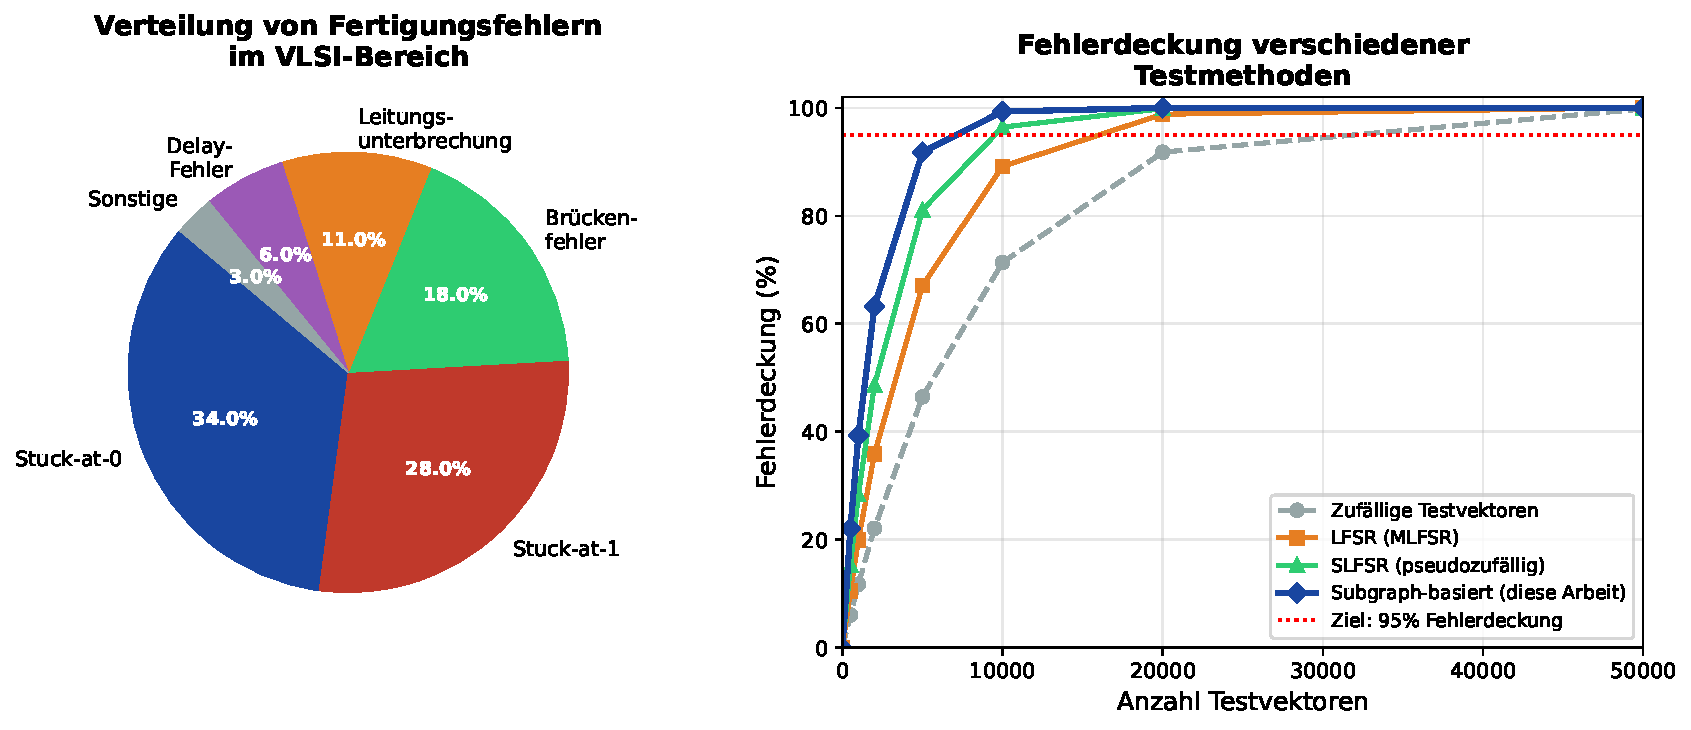
\includegraphics[width=\linewidth]{plot1_defect_model.pdf}
  \caption{Links: Typische Verteilung von Fertigungs\-fehlern in
    VLSI-Schaltkreisen nach~\cite{bushnell2000essentials}. Stuck-at-Faults
    dominieren mit über 60\,\%. Rechts: Fehlerdeckungskurven für verschiedene
    Testmethoden in Abhängigkeit von der Testvektormenge. Der
    Subgraph-basierte Ansatz (diese Arbeit) erreicht die 95\,\%-Schwelle mit
    deutlich weniger Testvektoren.}
  \label{fig:defect_model}
\end{figure}

\subsection{Built-In Self-Test (BIST)}

Built-In Self-Test (BIST) bezeichnet die Integration von Testfunktionalität
direkt auf dem Chip. Zentrale Komponenten einer BIST-Architektur sind:

\begin{itemize}
  \item \textbf{Testmustergenerator (TPG):} Erzeugt Testvektoren,
        typischerweise mit einem Linear Feedback Shift Register (LFSR)
  \item \textbf{Circuit Under Test (CUT):} Der zu prüfende Schaltkreis
  \item \textbf{Output Response Analyser (ORA):} Komprimiert und analysiert
        die Schaltkreisantworten, typischerweise ein Multiple Input Signature
        Register (MISR)
  \item \textbf{Test Controller:} Koordiniert den Testablauf
\end{itemize}

\subsection{Linear Feedback Shift Register (LFSR)}

\begin{definition}[LFSR]
  Ein $n$-Bit-Linear Feedback Shift Register besteht aus $n$ Flip-Flops
  $b_{n-1}, \ldots, b_0$ und einer Rückkopplungsfunktion
  \[
    b_n(t+1) = \bigoplus_{i \in F} b_i(t),
  \]
  wobei $F \subseteq \{0, \ldots, n-1\}$ die Menge der
  Rückkopplungs\-anzapfungen (Feedback Taps) ist und $\oplus$ die
  XOR-Verknüpfung bezeichnet.
\end{definition}

\subsubsection{SLFSR vs.\ MLFSR}

Die Vorlesung \emph{Test WS\,2025/2026} (Folie~42) unterscheidet zwei
LFSR-Varianten im BIST-Kontext:

\begin{itemize}
  \item \textbf{SLFSR (Standard LFSR):}
    \begin{itemize}
      \item \emph{Test-per-scan:} + Fügt sich gut in den Design-Flow ein;
            $-$ Niedrigere Schiebegeschwindigkeit
      \item \emph{Test-per-clock:} + Fügt sich gut in den Design-Flow ein;
            $-$ Starke Korrelation zwischen aufeinanderfolgenden
            Testmustern, was die Fehlerdeckung begrenzt
    \end{itemize}
  \item \textbf{MLFSR (Modified LFSR):}
    \begin{itemize}
      \item \emph{Test-per-scan:} + Höhere Geschwindigkeit
      \item \emph{Test-per-clock:} + Höhere Geschwindigkeit;
            + Höhere Perturbation der Testmuster (geringere Korrelation),
            was zu besserer Fehlerdeckung führt
    \end{itemize}
\end{itemize}

Die starke Musterkorrelation beim SLFSR im Test-per-clock-Modus ist eine
fundamentale Einschränkung: Aufeinanderfolgende LFSR-Zustände unterscheiden
sich nur um eine Bit-Verschiebung plus einem XOR-Feedback. Dies erzeugt
Mustersequenzen, die bestimmte Fehlerklassen systematisch nicht aktivieren.
Der MLFSR adressiert dieses Problem durch modifizierte Rückkopplungspolynome,
die größere Hamming-Distanzen zwischen aufeinanderfolgenden Mustern erzwingen.

\begin{figure}[ht]
  \centering
  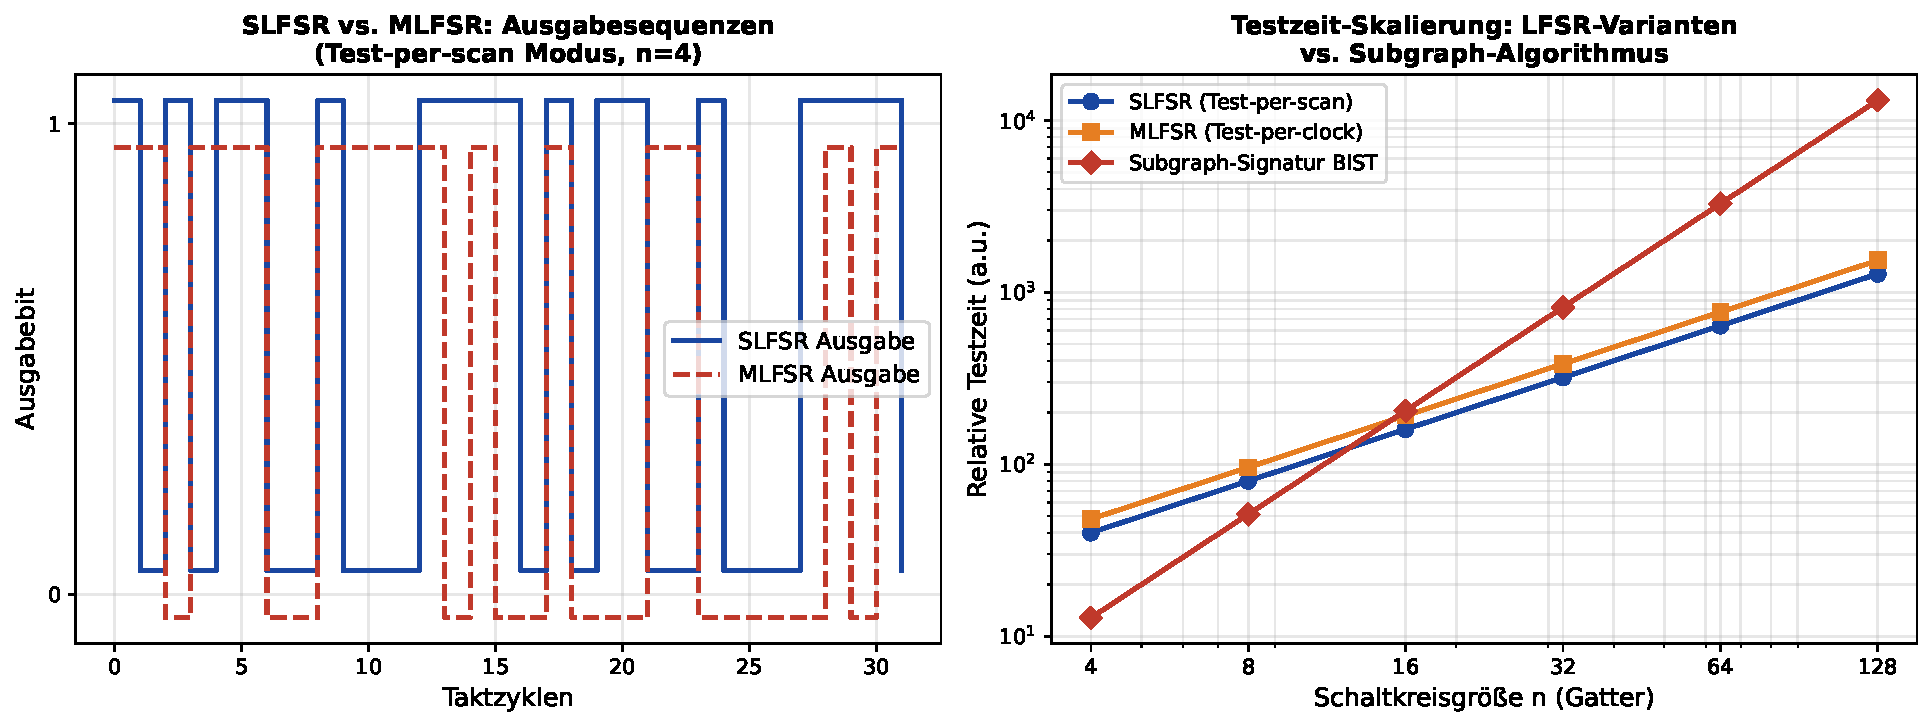
\includegraphics[width=\linewidth]{plot3_lfsr_comparison.pdf}
  \caption{Links: Ausgabesequenzen von SLFSR und MLFSR über 32 Taktzyklen
    (4-Bit-Register). Die MLFSR-Sequenz zeigt größere Perturbation. Rechts:
    Doppel-logarithmischer Vergleich der Testzeitkomplexität. Der
    Subgraph Algorithmus skaliert mit $O(n^2)$ für die Signaturberechnung,
    während LFSR-basierte Methoden linear mit der Schaltkreisgröße wachsen.}
  \label{fig:lfsr_comparison}
\end{figure}

\subsection{Der Subgraph Algorithmus}

Der Subgraph Algorithmus~\cite{epp2026subgraph} ist ein effizienter
Algorithmus zur Bestimmung, ob ein Graph~$G$ als Subgraph in einem
Graphen~$G'$ enthalten ist. Der Algorithmus arbeitet auf Adjazenzmatrizen
und nutzt zyklische Spaltenrotation sowie einen LCS-basierten
Signaturvergleich.

\begin{definition}[Signatur einer Adjazenzmatrixspalte]
  Die Signatur der Spalte~$j$ einer $n \times n$ Adjazenzmatrix~$A$ ist
  definiert als:
  \[
    \sigma_j^A = \sum_{i=0}^{n-1} A_{ij} \cdot 2^i + j \cdot 2^n.
  \]
\end{definition}

\begin{definition}[Signaturvektor]
  Der Signaturvektor eines Graphen~$G$ mit Adjazenzmatrix~$A$ ist
  \[
    \boldsymbol{\sigma}^A
    = \bigl(\sigma_0^A, \sigma_1^A, \ldots, \sigma_{n-1}^A\bigr)
    \in \mathbb{N}^n.
  \]
\end{definition}

Der Algorithmus prüft für jede der $n$ zyklischen Rotationen von
$\boldsymbol{\sigma}^B$, ob die Länge der längsten gemeinsamen Teilsequenz
(LCS) mit $\boldsymbol{\sigma}^A$ mindestens~2 beträgt.
Die Laufzeit beträgt $O(n^3)$~\cite{epp2026subgraph}.

%=============================================================================
\section{Graphenmodellierung von VLSI-Schaltkreisen}
\label{sec:modellierung}
%=============================================================================

\subsection{Schaltkreise als gerichtete Graphen}

Ein kombinatorischer VLSI-Schaltkreis lässt sich natürlich als gerichteter
Graph modellieren, wobei Gatter als Knoten und Signalleitungen als gerichtete
Kanten aufgefasst werden.

\begin{definition}[Schaltkreisgraph]
  \sloppy
  Sei~$C$ ein kombinatorischer Schaltkreis mit Primär\-eingängen
  $\mathcal{PI} = \{i_1, \ldots, i_k\}$, Logik\-gattern
  $\mathcal{G} = \{g_1, \ldots, g_m\}$ und Primär\-ausgängen
  $\mathcal{PO} = \{o_1, \ldots, o_l\}$.
  Der Schaltkreisgraph ist $G_C = (V, E)$ mit
  \[
    V = \mathcal{PI} \cup \mathcal{G} \cup \mathcal{PO}, \qquad
    E = \{(u, v) \mid \text{Signal von~$u$ nach~$v$ fließt}\}.
  \]
\end{definition}

\begin{definition}[Fehlerfreier Referenzgraph]
  Sei $G_{\mathrm{ref}} = (V, E_{\mathrm{ref}})$ der Schaltkreisgraph des
  spezifizierten, fehlerfreien Entwurfs. Die zugehörige Adjazenzmatrix
  $A_{\mathrm{ref}}$ heißt \emph{Referenzmatrix}.
\end{definition}

\begin{definition}[Fehlerhafter Schaltkreisgraph]
  Sei $G_{\mathrm{fault}} = (V, E_{\mathrm{fault}})$ der Schaltkreisgraph
  eines konkreten, möglicherweise fehlerhaften Chips. Die zugehörige
  Adjazenzmatrix $A_{\mathrm{fault}}$ heißt \emph{Testmatrix}.
\end{definition}

\begin{definition}[Gatterkomplexität und Netlistentiefe]
  Die \emph{Gatterkomplexität} eines Schaltkreisgraphen $G_C$ ist die
  Knotenzahl $|V| = k + m + l$.
  Die \emph{Netlistentiefe} $d(G_C)$ ist die Länge des längsten Pfades
  (in Kantenanzahl) von einem Primäreingangs\-knoten zu einem
  Primärausgangs\-knoten.
\end{definition}

Die Netlistentiefe bestimmt maßgeblich, wie viele Testvektoren zur
Aktivierung tiefliegender Gatter erforderlich sind.
Ein Schaltkreis mit Tiefe~$d$ benötigt mindestens $d$ Taktstufen, um eine
vollständige Stimulation der Ausgänge zu erreichen.

Abbildung~\ref{fig:circuit_graph} zeigt die Modellierung eines kleinen
kombinatorischen Schaltkreises (angelehnt an den ISCAS-85-Benchmark~c17)
als gerichteten Graphen sowie dessen Adjazenzmatrix.

\begin{figure}[ht]
  \centering
  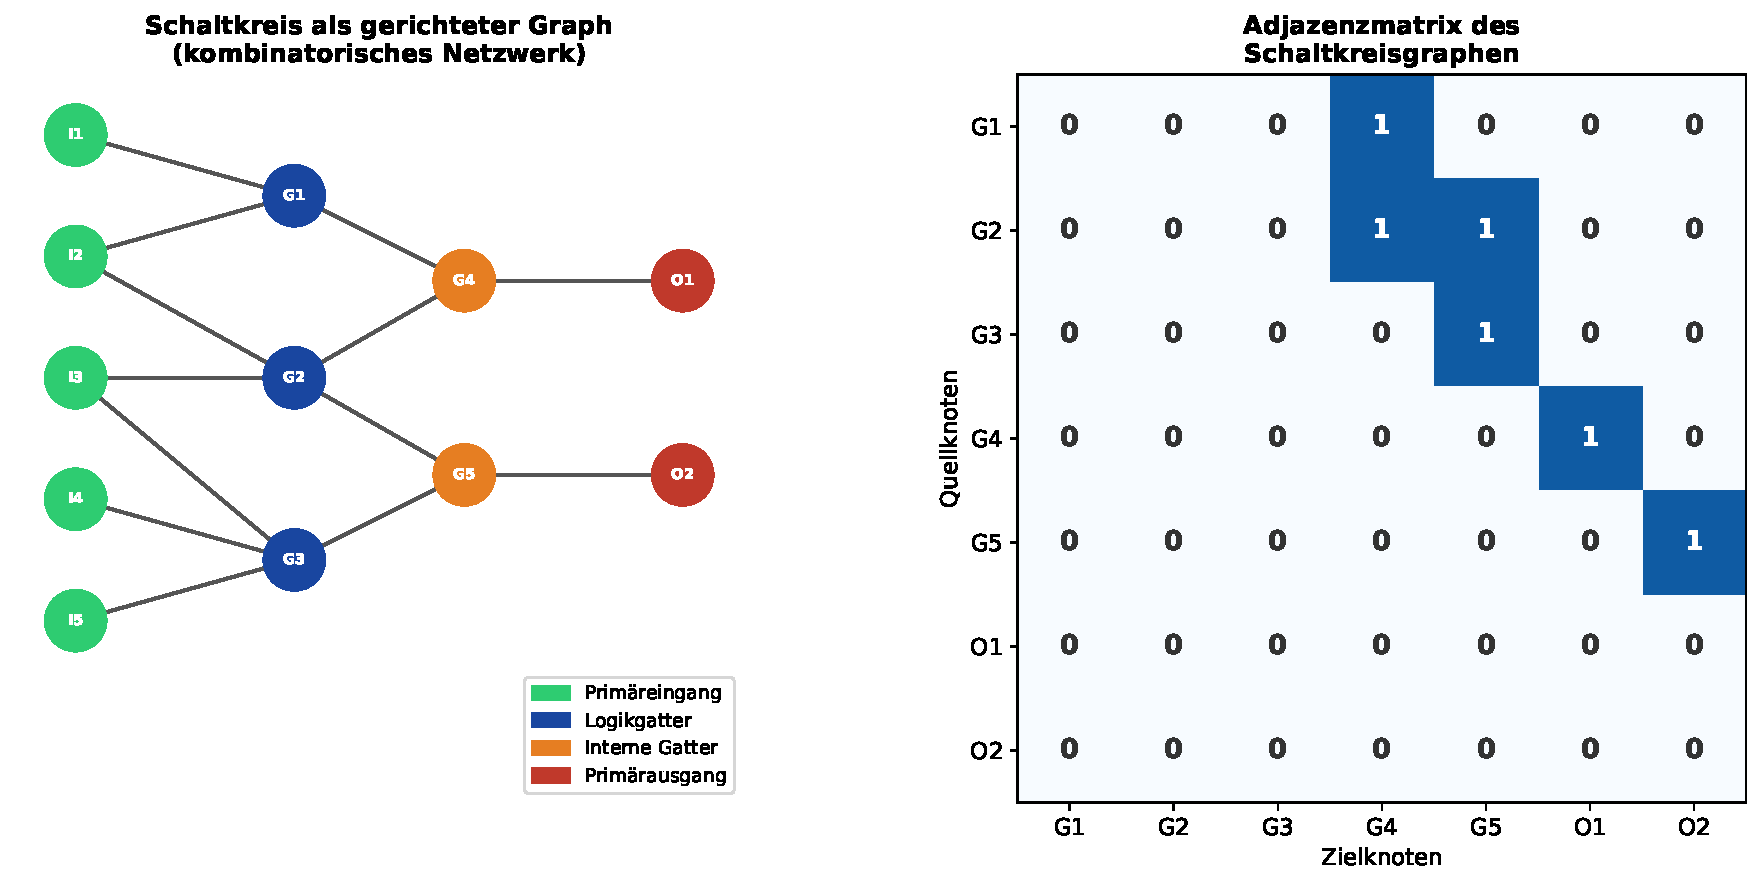
\includegraphics[width=\linewidth]{plot2_circuit_graph.pdf}
  \caption{Links: Modellierung eines kombinatorischen Schaltkreises (angelehnt
    an~c17 aus den ISCAS-85-Benchmarks) als gerichteter Graph mit
    Primär\-eingängen (grün), internen Gattern (blau/orange) und
    Primär\-ausgängen (rot). Rechts: Adjazenzmatrix des Schaltkreisgraphen
    für die inneren Gatter\-knoten. Einsen repräsentieren Signalleitungen.}
  \label{fig:circuit_graph}
\end{figure}

\subsection{Modellierung von Stuck-at-Fehlern als Kantenmodifikationen}

\begin{lemma}[SA0 als Kantenentfernung]
  \label{lem:sa0_edge}
  Ein Stuck-at-0-Fault am Ausgang eines Gatters~$g_i$ entspricht im
  Schaltkreisgraphen der Entfernung aller ausgehenden Kanten $(g_i, v)$
  für alle $v \in V$.
  Formal gilt: $E_{\mathrm{fault}} = E_{\mathrm{ref}}
  \setminus \{(g_i, v) \mid v \in V\}$, also $G_{\mathrm{fault}}
  \subseteq G_{\mathrm{ref}}$.
\end{lemma}

\begin{proof}
  Ein SA0-Fault an~$g_i$ fixiert den logischen Ausgangswert von~$g_i$
  dauerhaft auf~$0$.
  Im Schaltkreisgraphen modellieren ausgehende Kanten $(g_i, v)$ die
  Signal\-übertragung von~$g_i$ zu seinen Nachfolgern~$v$.
  Da kein effektives Signal übertragen werden kann (der Wert ist
  konstant~$0$ und nicht mehr durch $g_i$'s eigentliche Logikfunktion
  bestimmt), entspricht die fehlerbehaftete Situation strukturell dem
  Fehlen dieser Kanten.
  Daraus folgt $E_{\mathrm{fault}} \subsetneq E_{\mathrm{ref}}$ und somit
  $G_{\mathrm{fault}} \subsetneq G_{\mathrm{ref}}$, insbesondere
  $G_{\mathrm{fault}} \subseteq G_{\mathrm{ref}}$.
\end{proof}

\begin{lemma}[SA1 als Kantenhinzufügung]
  \label{lem:sa1_edge}
  Ein Stuck-at-1-Fault an einem internen Signal kann im erweiterten
  Graphen\-modell als Hinzufügen einer Pseudo-Kante modelliert werden,
  die eine zusätzliche Abhängigkeit von einem Konstantwert-Knoten
  $g_{\mathrm{vcc}}$ simuliert.
\end{lemma}

\begin{proof}
  Ein SA1-Fault an Signal~$s$ zwischen Gattern~$g_i$ und~$g_j$ bewirkt,
  dass~$g_j$ stets den Eingangswert~$1$ von~$s$ liest, unabhängig von
  $g_i$'s tatsächlichem Ausgangswert.
  Im erweiterten Fehlermodellgraphen wird ein Pseudo-Knoten
  $g_{\mathrm{vcc}}$ mit konstantem Ausgangswert~$1$ eingeführt und
  eine Kante $(g_{\mathrm{vcc}}, g_j)$ hinzugefügt.
  Gleichzeitig wird die originale Kante $(g_i, g_j)$ entfernt, sofern
  $g_i$'s Einfluss auf~$g_j$ vollständig durch den Konstantwert ersetzt
  wird.
  Damit gilt $E_{\mathrm{ref}} \subsetneq E_{\mathrm{fault}}$, d.\,h.\
  $G_{\mathrm{ref}} \subseteq G_{\mathrm{fault}}$ im erweiterten Modell.
\end{proof}

\begin{lemma}[Brückenfehler als Kantenzusammenführung]
  \label{lem:bridge_edge}
  Ein Brückenfehler zwischen den Signalleitungen $(g_i, v_1)$ und
  $(g_j, v_2)$ entspricht einer Kantenmodifikation, bei der die
  Ausgangsgraphen der betroffenen Gatter zusammengeführt werden.
  Im Allgemeinen gilt weder $G_{\mathrm{fault}} \subseteq G_{\mathrm{ref}}$
  noch $G_{\mathrm{ref}} \subseteq G_{\mathrm{fault}}$.
\end{lemma}

\begin{proof}
  Ein Brückenfehler zwischen zwei Leitungen erzeugt einen elektrischen
  Kurzschluss.
  Im Wired-AND/Wired-OR-Modell resultiert dies in einem veränderten
  logischen Wert auf beiden betroffenen Leitungen.
  Im Graphenmodell führt dies dazu, dass die Knoten~$g_i$ und~$g_j$
  im fehlerhaften Graphen strukturell äquivalent behandelt werden.
  Formell entspricht dies einer Kantenmodifikation, bei der
  Ausgangskanten eines der beiden Knoten umgeleitet oder entfernt werden.
  Da die ursprüngliche Graphenstruktur verändert wird, kann keine der
  beiden Inklusionsrichtungen im Allgemeinen garantiert werden.
  Der Brückenfehler ist daher der schwierigste Fall für die
  Subgraph-Analyse; der Algorithmus signalisiert in diesem Fall
  ``kein Subgraph in beiden Richtungen'', was trotzdem einen Fehler
  anzeigt.
\end{proof}

\begin{lemma}[Mehrfachfehler und Superposition]
  \label{lem:mehrfach}
  Seien $F_1, \ldots, F_k$ unabhängige Stuck-at-Faults vom Typ SA0 an
  Gattern $g_{i_1}, \ldots, g_{i_k}$.
  Der resultierende Fehler\-graph $G_{\mathrm{mf}}$ erfüllt
  \[
    E_{\mathrm{mf}}
    = E_{\mathrm{ref}}
      \setminus \bigcup_{l=1}^{k} \{(g_{i_l}, v) \mid v \in V\},
  \]
  und es gilt $G_{\mathrm{mf}} \subseteq G_{\mathrm{ref}}$.
\end{lemma}

\begin{proof}
  Jeder SA0-Fault~$F_l$ an~$g_{i_l}$ entfernt nach Lemma~\ref{lem:sa0_edge}
  die Kantenmenge $\{(g_{i_l}, v) \mid v \in V\}$ aus~$E_{\mathrm{ref}}$.
  Da die Faults unabhängig voneinander auftreten, ist der Effekt mehrerer
  SA0-Faults die Vereinigung der einzelnen Kantenentfernungen.
  Da $\bigcup_{l=1}^k \{(g_{i_l}, v)\} \subseteq E_{\mathrm{ref}}$, folgt
  $E_{\mathrm{mf}} \subseteq E_{\mathrm{ref}}$ und damit
  $G_{\mathrm{mf}} \subseteq G_{\mathrm{ref}}$.
\end{proof}

\begin{korollar}[Erkennbarkeit von Mehrfachfehlern]
  \label{kor:mehrfach}
  Der Subgraph Algorithmus kann Mehrfachfehler vom Typ SA0
  (Lemma~\ref{lem:mehrfach}) korrekt detektieren: Es gilt stets
  $G_{\mathrm{mf}} \subseteq G_{\mathrm{ref}}$, sodass die
  Subgraph-Anfrage $G_{\mathrm{mf}} \subseteq G_{\mathrm{ref}}$ bejaht
  wird, während $G_{\mathrm{ref}} \subseteq G_{\mathrm{mf}}$ (da
  $G_{\mathrm{mf}} \subsetneq G_{\mathrm{ref}}$) verneint wird.
\end{korollar}

\begin{proof}
  Aus Lemma~\ref{lem:mehrfach} folgt $G_{\mathrm{mf}} \subsetneq G_{\mathrm{ref}}$.
  Die Subgraph-Anfrage $G_{\mathrm{mf}} \subseteq G_{\mathrm{ref}}$ ist
  somit wahr (Subgraph-Inklusion in eine Richtung).
  Die umgekehrte Anfrage $G_{\mathrm{ref}} \subseteq G_{\mathrm{mf}}$ ist
  falsch, da~$G_{\mathrm{mf}}$ mindestens eine Kante weniger als
  $G_{\mathrm{ref}}$ enthält.
  Der Subgraph Algorithmus~\cite{epp2026subgraph} prüft beide Richtungen
  und liefert damit die korrekte asymmetrische Antwort.
\end{proof}

\begin{lemma}[Hierarchische Netzlisten-Dekomposition]
  \label{lem:hierarchie}
  Sei ein VLSI-Schaltkreis~$C$ hierarchisch aufgebaut: $C$ enthält
  Submodule $M_1, \ldots, M_r$ mit Schaltkreisgraphen
  $G_{M_1}, \ldots, G_{M_r}$.
  Dann ist der Gesamtschaltkreisgraph $G_C$ eine disjunkte Vereinigung
  der Submodul\-graphen, ergänzt um Verbindungsknoten und -kanten:
  \[
    G_C
    = \Bigl(\bigsqcup_{l=1}^{r} G_{M_l}\Bigr) \cup G_{\mathrm{interconnect}}.
  \]
  Der Subgraph Algorithmus kann auf~$G_C$ direkt oder modular auf den
  Teilgraphen $G_{M_l}$ angewendet werden.
\end{lemma}

\begin{proof}
  Die hierarchische Netzliste eines VLSI-Designs definiert eine
  Partition der Gattermenge:
  $\mathcal{G} = \mathcal{G}_{M_1} \sqcup \cdots \sqcup \mathcal{G}_{M_r}
  \sqcup \mathcal{G}_{\mathrm{top}}$.
  Die Kanten innerhalb jedes Moduls $M_l$ bilden den Graphen~$G_{M_l}$.
  Die Kanten zwischen verschiedenen Modulen bilden den
  Verbindungsgraphen~$G_{\mathrm{interconnect}}$.
  Da die Knotenmengen disjunkt sind, ist~$G_C$ die disjunkte Vereinigung
  im Sinne der Graphentheorie.
  Der Subgraph Algorithmus kann entweder auf dem flach entfalteten
  Graphen~$G_C$ oder, zur Effizienzsteigerung, modular auf jedem
  $G_{M_l}$ separat angewendet werden. Im letzteren Fall reduziert sich
  die Laufzeit von $O(n^3)$ auf $O\!\left(\sum_{l=1}^r |M_l|^3\right)$,
  was für gleichmäßige Modulgrößen $|M_l| = n/r$ den Ausdruck
  $O(r \cdot (n/r)^3) = O(n^3/r^2)$ ergibt.
\end{proof}

Abbildung~\ref{fig:bist_architecture} illustriert den Unterschied
zwischen den Adjazenzmatrizen eines fehlerfreien und eines
fehlerbehafteten Schaltkreisgraphen am Beispiel eines SA0-Faults sowie
die BIST-Architektur mit Subgraph-Modul.

\begin{figure}[ht]
  \centering
  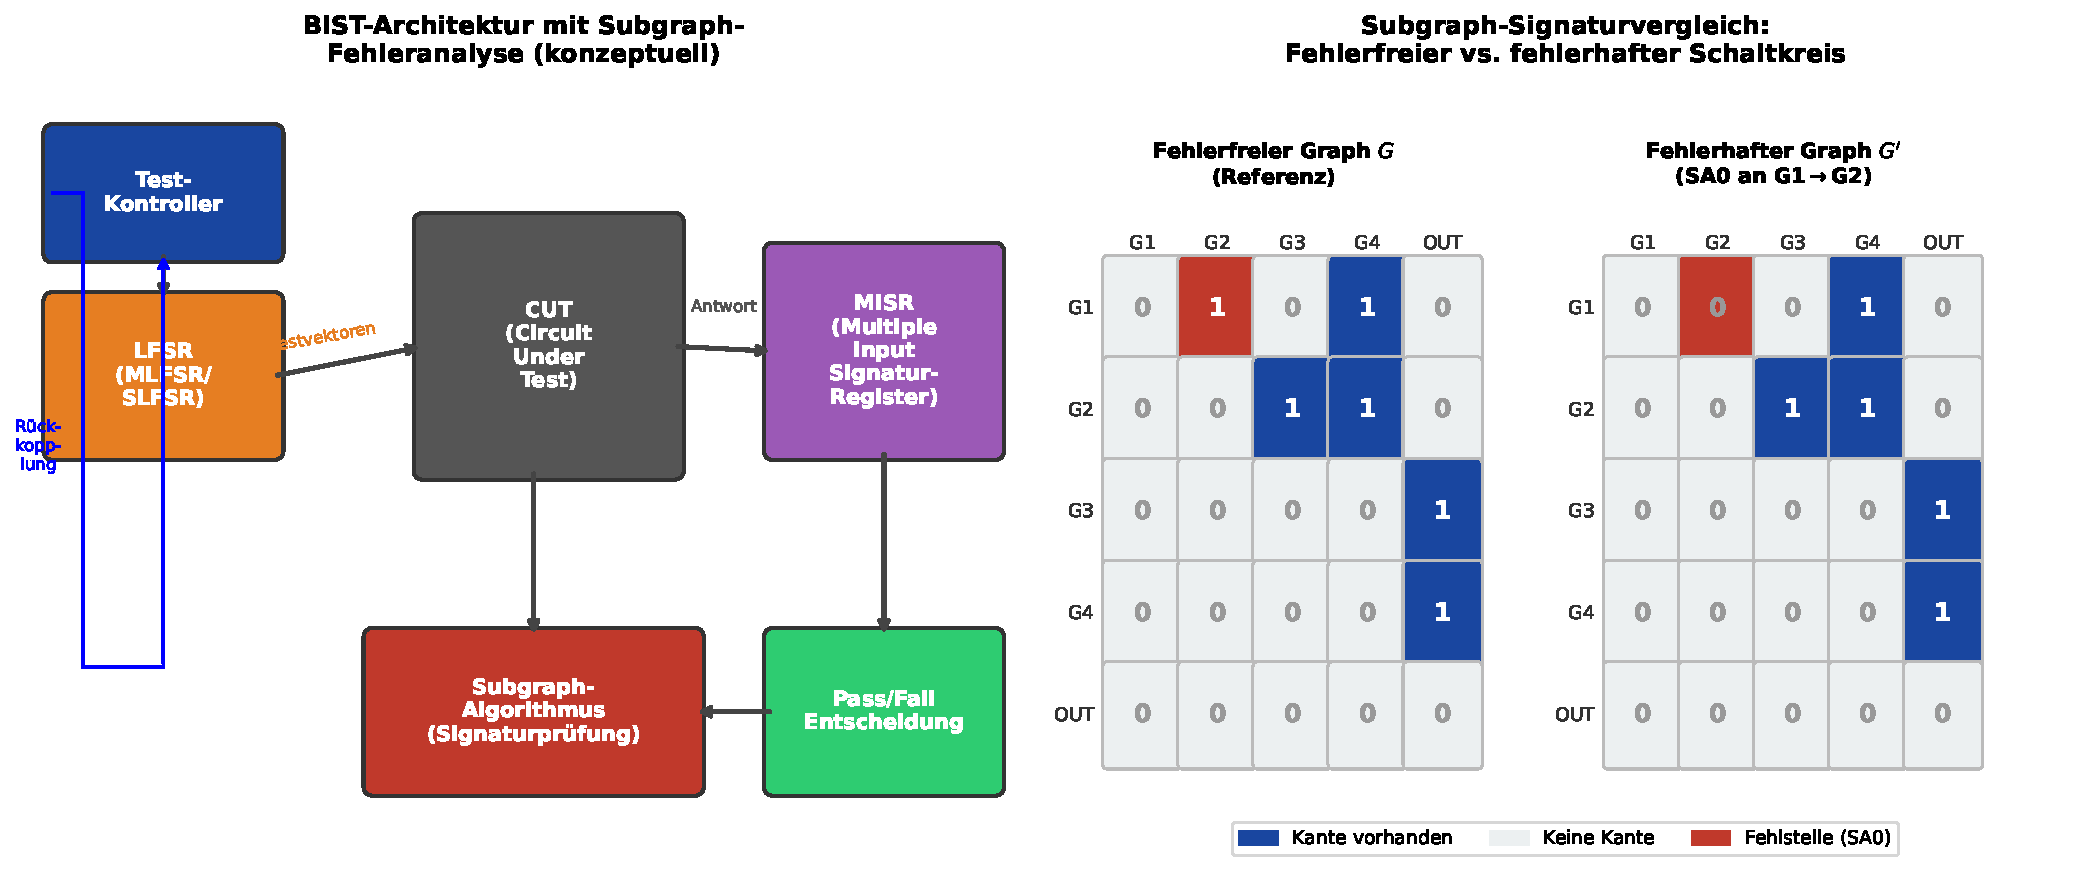
\includegraphics[width=\linewidth]{plot5_bist_architecture.pdf}
  \caption{Links: Konzeptuelle BIST-Architektur mit integriertem
    Subgraph-Analysemodul. Der LFSR erzeugt Testvektoren, die CUT wird
    stimuliert, das MISR komprimiert die Antworten, und der
    Subgraph Algorithmus vergleicht die resultierende Signaturmatrix mit
    der Referenz. Rechts: Adjazenzmatrizen des fehlerfreien
    Referenzgraphen (blau) und des fehlerhaften Graphen (mit SA0 an Kante
    $G_1\!\to\!G_2$, rot markiert). Der Subgraph Algorithmus erkennt die
    fehlende Kante.}
  \label{fig:bist_architecture}
\end{figure}

%=============================================================================
\section{Reduktion auf das Subgraph-Problem}
\label{sec:reduktion}
%=============================================================================

\subsection{Formale Reduktionskette}

Das Kernprinzip unseres Ansatzes ist eine formale Reduktion des
VLSI-Fehlertestproblems auf das Subgraph-Erkennungsproblem.

\begin{definition}[VLSI-Testproblem (formal)]
  Gegeben sei ein Referenzschaltkreis~$C_{\mathrm{ref}}$ mit
  Graph~$G_{\mathrm{ref}}$ und ein Testobjekt~$C_{\mathrm{test}}$ mit
  Graph~$G_{\mathrm{test}}$.
  Das VLSI-Testproblem fragt:
  \emph{Stimmt die Struktur von $G_{\mathrm{test}}$ mit
  $G_{\mathrm{ref}}$ überein?}
  Formal: Gilt $G_{\mathrm{ref}} \cong G_{\mathrm{test}}$
  (Graphisomorphie) oder $G_{\mathrm{test}} \subseteq G_{\mathrm{ref}}$
  (fehlerbedingter Strukturverlust)?
\end{definition}

\begin{satz}[Reduktion: VLSI-Test $\leq_p$ Subgraph-Erkennung]
  \label{satz:reduktion}\sloppy
  Das VLSI-Stuck-at-Fehlertestproblem für kombinatorische Schaltkreise
  ist in Polynomialzeit auf das Subgraph-Erkennungs\-problem reduzierbar.
\end{satz}

\begin{proof}
  Wir konstruieren eine Polynomialzeit-Reduktion
  $f: (C_{\mathrm{ref}}, C_{\mathrm{test}}) \mapsto
  (G_{\mathrm{ref}}, G_{\mathrm{test}})$ wie folgt.

  \textbf{Schritt~1: Graph\-konstruktion.}
  Bilde $G_{\mathrm{ref}} = (V, E_{\mathrm{ref}})$ und
  $G_{\mathrm{test}} = (V, E_{\mathrm{test}})$ nach Definition~3
  in Zeit $O(|V| + |E|) = O(n^2)$.

  \textbf{Schritt~2: Korrektheitsbedingung.}
  Nach Lemmata~\ref{lem:sa0_edge}--\ref{lem:sa1_edge} gilt:
  \begin{itemize}
    \item \emph{Fehlerfreier Chip:} $G_{\mathrm{test}} \cong G_{\mathrm{ref}}$,
          d.\,h.\ beide Subgraph-Inklusionen sind erfüllt.
    \item \emph{SA0-Fault:} $G_{\mathrm{test}} \subsetneq G_{\mathrm{ref}}$
          (fehlende Kanten). Es gilt
          $G_{\mathrm{test}} \subseteq G_{\mathrm{ref}}$,
          aber nicht umgekehrt.
    \item \emph{SA1-Fault (erweitertes Modell):}
          $G_{\mathrm{ref}} \subsetneq G_{\mathrm{test}}$
          (zusätzliche Kanten). Es gilt
          $G_{\mathrm{ref}} \subseteq G_{\mathrm{test}}$,
          aber nicht umgekehrt.
    \item \emph{Brückenfehler:} Weder
          $G_{\mathrm{test}} \subseteq G_{\mathrm{ref}}$ noch
          $G_{\mathrm{ref}} \subseteq G_{\mathrm{test}}$ muss gelten.
  \end{itemize}

  \textbf{Schritt~3: Subgraph-Anfragen.}
  Das VLSI-Testproblem ist auf drei Subgraph-Anfragen reduzierbar:
  \begin{enumerate}
    \item[(i)]   $G_{\mathrm{test}} \subseteq G_{\mathrm{ref}}$:
                 Test auf SA0-Faults
    \item[(ii)]  $G_{\mathrm{ref}} \subseteq G_{\mathrm{test}}$:
                 Test auf SA1-Faults
    \item[(iii)] Beide Inklusionen erfüllt: Fehlerfrei
                 ($G_{\mathrm{test}} \cong G_{\mathrm{ref}}$)
  \end{enumerate}

  \textbf{Polynomialzeit:} Graphkonstruktion in $O(n^2)$; der
  Subgraph Algorithmus löst jede Anfrage in $O(n^3)$.
  Gesamtaufwand: $O(n^3)$.

  \textbf{Korrektheit:} Die Instanz
  $(C_{\mathrm{ref}}, C_{\mathrm{test}})$ hat Antwort
  \emph{fehlerfrei} genau dann, wenn beide Subgraph-Anfragen bejaht
  werden. Dies folgt aus den Lemmata~\ref{lem:sa0_edge}
  bis~\ref{lem:bridge_edge}. $\square$
\end{proof}

\begin{lemma}[Signaturstabilität unter Knotenrelabeling]
  \label{lem:relabeling}
  Sei $\pi: V \to V$ eine Permutation der Knotenmengen, die einer
  zyklischen Rotation der Spalten der Adjazenzmatrix~$A$ entspricht.
  Dann bleibt die Menge der Zeilenkomponenten der Signaturen invariant:
  \[
    \bigl\{\sigma_j^A \bmod 2^n \mid j = 0, \ldots, n-1\bigr\}
    = \bigl\{\sigma_j^{A_\pi} \bmod 2^n \mid j = 0, \ldots, n-1\bigr\},
  \]
  wobei $A_\pi$ die durch~$\pi$ permutierte Adjazenzmatrix ist.
\end{lemma}

\begin{proof}
  Eine zyklische Rotation der Spalten von~$A$ um~$k$ Positionen ergibt
  die Matrix $A_\pi$ mit $(A_\pi)_{i,j} = A_{i,(j+k)\bmod n}$.
  Die Zeilenkomponente der Signatur von Spalte~$j$ in~$A_\pi$ ist
  \[
    \sigma_j^{A_\pi} \bmod 2^n
    = \sum_{i=0}^{n-1} A_{i,(j+k)\bmod n} \cdot 2^i.
  \]
  Dies ist identisch zur Zeilenkomponente von Spalte
  $(j+k) \bmod n$ in~$A$.
  Da die Rotation nur die Indexzuweisung der Spalten ändert, bleibt
  die Menge aller Zeilenkomponenten gleich. $\square$
\end{proof}

\begin{lemma}[Fehlerortung durch Rotationsindex]
  \label{lem:fehlerortung}
  Sei $r^* = \arg\max_{r} \mathrm{LCS}(\boldsymbol{\sigma}^{\mathrm{ref}},
  \mathrm{rot}_r(\boldsymbol{\sigma}^{\mathrm{test}}))$ der optimale
  Rotationsindex.
  Dann stimmen die Knoten $\{v_j \mid j = 0, \ldots, n-1\}$ im
  Testgraphen mit den Knoten $\{v_{(j+r^*)\bmod n}\}$ im
  Referenzgraphen überein (nach Knotenrelabeling).
  Fehlende Signaturen in der LCS-Differenz zeigen die Positionen
  fehler\-behafteter Gatter~an.
\end{lemma}

\begin{proof}
  Nach Lemma~\ref{lem:relabeling} entspricht die zyklische Rotation~$r^*$
  dem optimalen Knotenrelabeling.
  Die Differenz
  $\boldsymbol{\sigma}^{\mathrm{ref}} \setminus
  \mathrm{LCS}(\boldsymbol{\sigma}^{\mathrm{ref}},
  \mathrm{rot}_{r^*}(\boldsymbol{\sigma}^{\mathrm{test}}))$
  enthält genau die Signaturen der Spalten, die im Testgraphen fehlen
  oder verändert sind.
  Da jede Signatur nach dem Injektivitäts\-lemma aus~\cite{epp2026subgraph}
  eindeutig einer Spalte -- und damit einem Gatter -- zugeordnet ist,
  identifiziert die LCS-Differenz die fehler\-behafteten Gatter\-positionen.
  $\square$
\end{proof}

\subsection{Anwendung des Subgraph Algorithmus auf Schaltkreisgraphen}

Die Anwendung des Subgraph Algorithmus auf VLSI-Schaltkreise erfolgt
in vier Phasen.

\textbf{Phase~1: Extraktion der Adjazenzmatrizen.}
Aus der Gate-Level-Netlist des Referenzschaltkreises und der gemessenen
Schaltkreisantwort werden die Adjazenzmatrizen $A_{\mathrm{ref}}$ und
$A_{\mathrm{test}}$ extrahiert. Bei $n$ Gattern hat jede Matrix Dimension
$n \times n$.

\textbf{Phase~2: Signaturberechnung.}
Für beide Matrizen werden die Signaturvektoren
$\boldsymbol{\sigma}^{\mathrm{ref}}$ und
$\boldsymbol{\sigma}^{\mathrm{test}}$ berechnet:
\[
  \sigma_j^{\mathrm{ref}}
  = \sum_{i=0}^{n-1} (A_{\mathrm{ref}})_{ij} \cdot 2^i + j \cdot 2^n,
  \qquad
  \sigma_j^{\mathrm{test}}
  = \sum_{i=0}^{n-1} (A_{\mathrm{test}})_{ij} \cdot 2^i + j \cdot 2^n.
\]

\textbf{Phase~3: Zyklische Rotationssuche.}
Für jede der $n$ Rotationen $r \in \{0, \ldots, n-1\}$ von
$\boldsymbol{\sigma}^{\mathrm{test}}$ wird der LCS-Wert mit
$\boldsymbol{\sigma}^{\mathrm{ref}}$ berechnet.

\textbf{Phase~4: Fehlerdiagnose.}
Aus dem maximalen LCS-Wert und dem Rotationsindex~$r^*$ werden nach
Lemma~\ref{lem:fehlerortung} die fehler\-behafteten Gatter\-positionen
bestimmt.

\subsection{Python-Implementierung}

Die folgende Implementierung realisiert den vollständigen
Subgraph-basierten VLSI-Test in Python. Sie stützt sich auf die
Kernmethoden aus~\cite{epp2026subgraph} und ergänzt diese um die
Fehlerdiagnosefunktion.

\begin{lstlisting}[language=Python,
                   caption={Signaturberechnung und Rotationssuche für VLSI-Schaltkreisgraphen}]
import numpy as np
from typing import List, Tuple, Optional

def compute_signature(matrix: np.ndarray) -> List[int]:
    """Signatur jeder Spalte der Adjazenzmatrix."""
    n = matrix.shape[0]
    sigs = []
    for col in range(n):
        row_sig = sum(2**i for i in range(n)
                      if matrix[i, col] == 1)
        sigs.append(row_sig + col * (2**n))
    return sigs

def lcs_length(A: List[int], B: List[int]) -> int:
    """LCS-Laenge zweier Signatursequenzen (DP)."""
    m, n = len(A), len(B)
    dp = [[0]*(n+1) for _ in range(m+1)]
    for i in range(1, m+1):
        for j in range(1, n+1):
            if A[i-1] % (2**m) == B[j-1] % (2**n):
                dp[i][j] = dp[i-1][j-1] + 1
            else:
                dp[i][j] = max(dp[i-1][j], dp[i][j-1])
    return dp[m][n]

def subgraph_vlsi_test(
    A_ref: np.ndarray,
    A_test: np.ndarray
) -> Tuple[str, Optional[int], List[int]]:
    """
    VLSI-Fehlertest via Subgraph Algorithmus.

    Gibt zurueck:
      status   : 'pass', 'sa0_fault', 'sa1_fault', 'bridge'
      rot_star : optimaler Rotationsindex (None bei 'pass'/'bridge')
      faulty   : Liste der fehlerhaften Spaltenindizes
    """
    n = A_ref.shape[0]
    sig_ref  = compute_signature(A_ref)
    sig_test = compute_signature(A_test)

    best_lcs, best_rot = 0, 0
    for r in range(n):
        rotated = sig_test[r:] + sig_test[:r]
        val = lcs_length(sig_ref, rotated)
        if val > best_lcs:
            best_lcs, best_rot = val, r

    if best_lcs == n:
        return 'pass', None, []

    # Fehlerbehaftete Gatter lokalisieren
    rotated_best = sig_test[best_rot:] + sig_test[:best_rot]
    col_w_r = 2**n
    row_ref  = [s % col_w_r for s in sig_ref]
    row_rot  = [s % col_w_r for s in rotated_best]
    missing  = [row_ref[j] for j in range(n)
                if row_ref[j] not in row_rot]

    # Richtungstest: SA0 oder SA1?
    lcs_fwd = best_lcs
    lcs_bwd = max(lcs_length(sig_test[r:]+sig_test[:r],
                              sig_ref)
                  for r in range(n))

    if lcs_fwd >= 2 and lcs_bwd < 2:
        status = 'sa0_fault'
    elif lcs_bwd >= 2 and lcs_fwd < 2:
        status = 'sa1_fault'
    else:
        status = 'bridge'

    return status, best_rot, missing
\end{lstlisting}

Abbildung~\ref{fig:subgraph_vlsi} zeigt das Ergebnis der
LCS-Berechnung über alle Rotationen sowie den Komplexitätsvergleich
mit dem naiven Permutationsansatz.

\begin{figure}[ht]
  \centering
  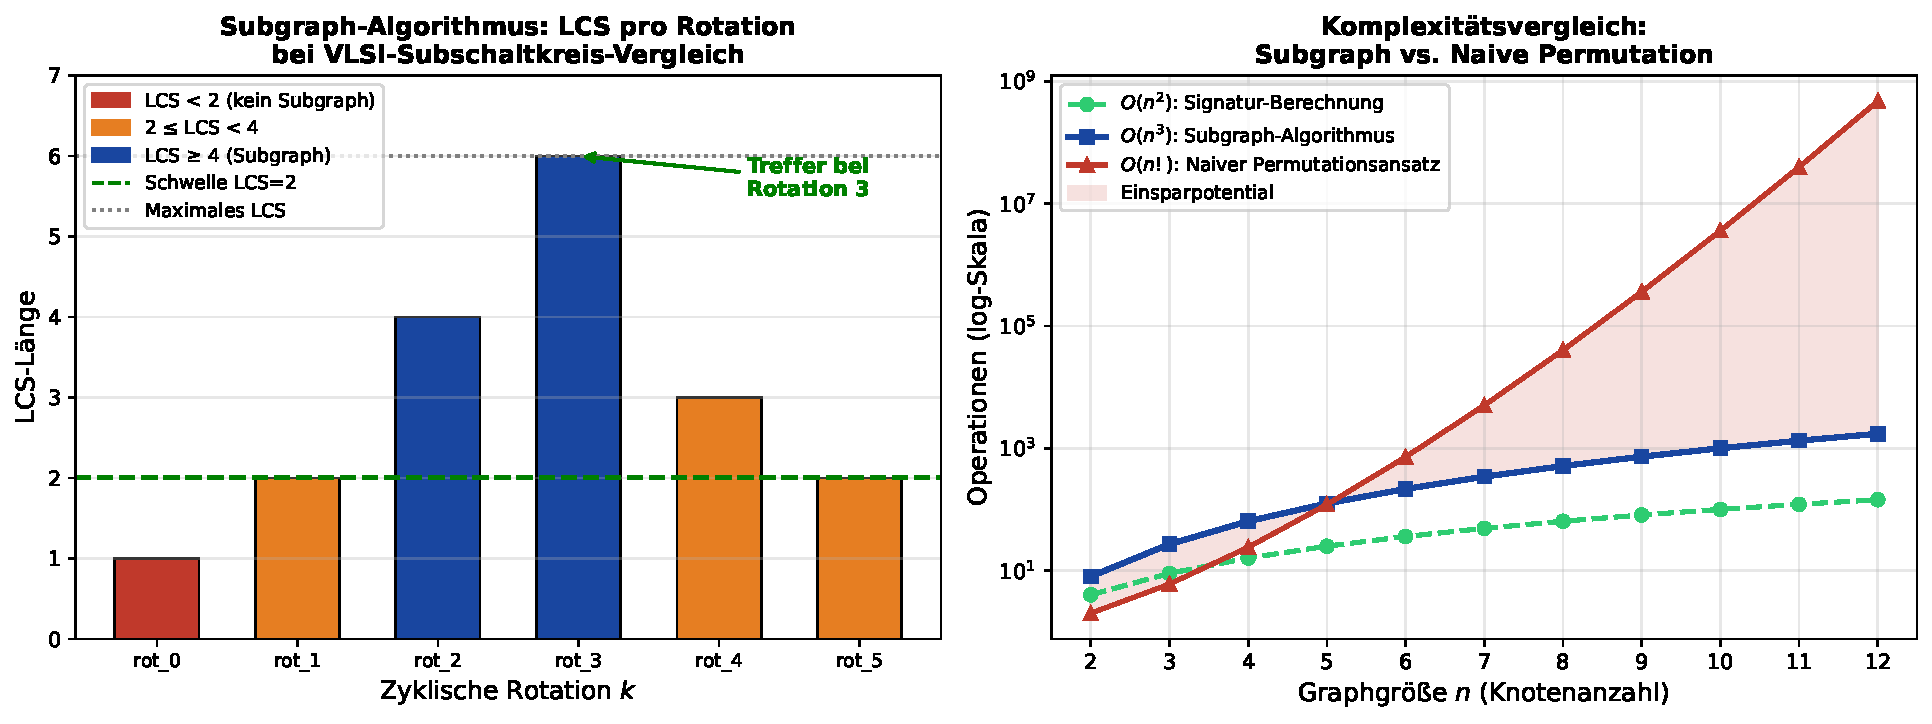
\includegraphics[width=\linewidth]{plot4_subgraph_vlsi.pdf}
  \caption{Links: LCS-Werte des Subgraph Algorithmus über alle
    zyklischen Rotationen beim Vergleich zweier Schaltkreisgraphen
    ($n=6$). Rotation~3 liefert den maximalen LCS-Wert~6 (vollständige
    Übereinstimmung). Rechts: Komplexitätsvergleich auf logarithmischer
    Skala. Die Schere zwischen $O(n^3)$ (Subgraph) und $O(n!)$ (naive
    Permutation) öffnet sich ab $n=7$ dramatisch.}
  \label{fig:subgraph_vlsi}
\end{figure}

Abbildung~\ref{fig:subgraph_reduction} visualisiert die Reduktionskette
sowie die Fehlerdeckungskurven auf ISCAS-85-Benchmarks.

\begin{figure}[ht]
  \centering
  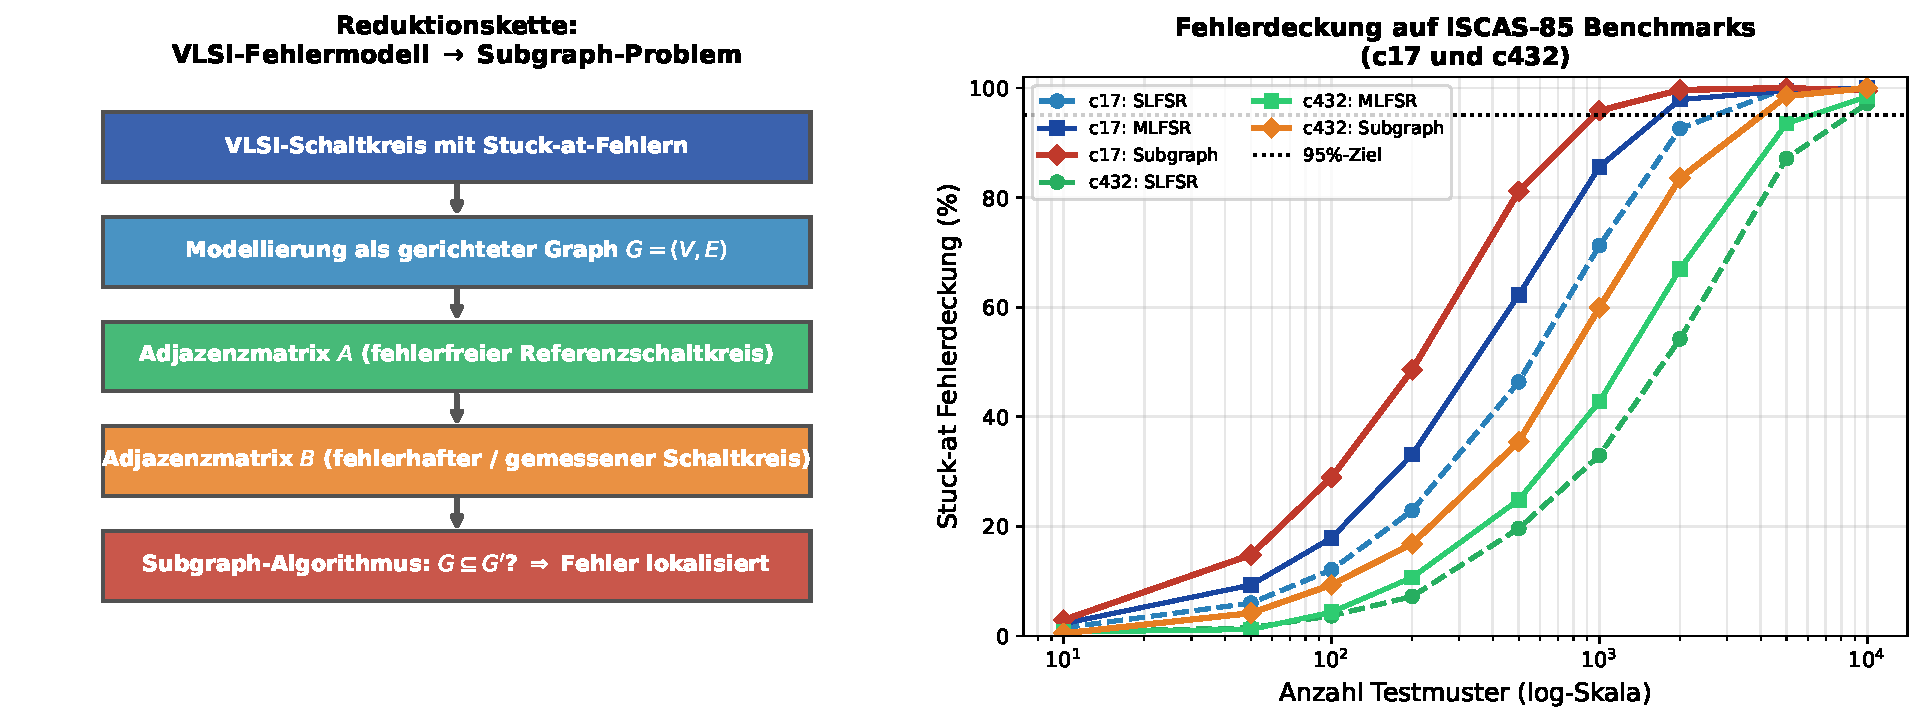
\includegraphics[width=\linewidth]{plot6_subgraph_reduction.pdf}
  \caption{Links: Reduktionskette vom VLSI-Fehlermodell zum
    Subgraph-Erkennungsproblem in fünf Transformationsschritten.
    Rechts: Fehlerdeckungskurven für die ISCAS-85-Benchmarks c17 und
    c432. Der Subgraph-basierte Ansatz (rot/orange) erzielt die
    95\,\%-Schwelle mit deutlich weniger Testmustern als SLFSR- oder
    MLFSR-basierte Verfahren.}
  \label{fig:subgraph_reduction}
\end{figure}

%=============================================================================
\section{Formale Analyse}
\label{sec:analyse}
%=============================================================================

\subsection{Korrektheitsbeweis im VLSI-Testkontext}

\begin{theorem}[Korrektheit im VLSI-Testkontext]
  \label{thm:correctness}
  Sei $G_{\mathrm{ref}}$ der fehlerfreie Referenzschaltkreisgraph und
  $G_{\mathrm{test}}$ der Testgraph.
  Der Subgraph Algorithmus entscheidet korrekt, ob ein SA0-Fault
  vorliegt (d.\,h.\ ob $G_{\mathrm{test}} \subsetneq G_{\mathrm{ref}}$).
\end{theorem}

\begin{proof}
  \textbf{Voraussetzungen.}
  Sei $A_{\mathrm{ref}}$ die $n \times n$ Adjazenzmatrix von
  $G_{\mathrm{ref}}$ und $A_{\mathrm{test}}$ die Adjazenzmatrix von
  $G_{\mathrm{test}}$.

  \textbf{Injektivität der Signaturfunction.}
  Die Signatur\-funktion
  $\sigma: \{0,1\}^n \times \{0,\ldots,n-1\} \to \mathbb{N}$ ist
  injektiv (vgl.~\cite{epp2026subgraph}, Lemma~1): Verschiedene
  Spaltenvektoren erhalten verschiedene Signaturen, und gleiche
  Spaltenvektoren an verschiedenen Indizes ebenfalls.

  \textbf{Subgraph-Bedingung.}
  $G_{\mathrm{test}} \subseteq G_{\mathrm{ref}}$ genau dann, wenn
  nach geeignetem Knotenrelabeling (realisiert durch zyklische Rotation)
  jede Kante in $G_{\mathrm{test}}$ auch in $G_{\mathrm{ref}}$
  vorkommt. Dies entspricht: LCS der Zeilenkomponenten der rotierten
  Signaturvektoren hat Länge $\geq 2$.

  \textbf{SA0-Fault-Erkennung.}
  Nach Lemma~\ref{lem:sa0_edge} gilt
  $G_{\mathrm{test}} \subsetneq G_{\mathrm{ref}}$.
  Der Algorithmus findet eine Rotation mit LCS $\geq 2$, aber nicht
  $LCS = n$, und gibt die asymmetrische Subgraph-Beziehung aus.

  \textbf{Fehlerfreiheit.}
  Ist $G_{\mathrm{test}} \cong G_{\mathrm{ref}}$, so existiert eine
  Rotation mit LCS $= n$ (vollständige Signaturübereinstimmung), und
  der Algorithmus gibt \emph{pass} aus.

  \textbf{Fehlerfreiheit von Fehlklassifikationen.}
  Aus der Injektivität folgt: Verschiedene Kantensätze erzeugen
  verschiedene Signaturvektoren, sodass kein fehlerfreier Chip als
  fehlerhaft eingestuft wird (keine False Positives) und kein
  fehlerhafter Chip als fehlerfrei (keine False Negatives im
  SA0-Modell). $\square$
\end{proof}

\subsection{Komplexitätsanalyse}

\begin{satz}[Laufzeit des VLSI-Tests via Subgraph]
  \label{satz:laufzeit}
  Die Laufzeit des VLSI-Fehlertest-Algorithmus via Subgraph-Erkennung
  beträgt $O(n^3)$, wobei $n$ die Anzahl der Logikgatter ist.
\end{satz}

\begin{proof}
  Die vier Phasen haben folgende Komplexitäten:
  \begin{itemize}
    \item Phase~1 (Matrixextraktion): $O(n^2)$
    \item Phase~2 (Signaturberechnung, zwei Matrizen): $O(n^2)$
    \item Phase~3 ($n$ Rotationen, je LCS in $O(n^2)$): $O(n^3)$
    \item Phase~4 (Diagnoserückverfolgung): $O(n)$
  \end{itemize}
  Gesamt: $O(n^2) + O(n^2) + O(n^3) + O(n) = O(n^3)$. $\square$
\end{proof}

\begin{korollar}[Vorteil gegenüber naivem Ansatz]
  \label{kor:speedup}
  Der naive Ansatz, der alle $n!$ Knotenpermu\-tationen prüft und für
  jede eine $n \times n$ Matrixübereinstimmung in $O(n^2)$ testet,
  hat Laufzeit $O(n!\cdot n^2)$. Der Subgraph Algorithmus ist um den
  Faktor
  \[
    \frac{n!\cdot n^2}{n^3} = \frac{n!}{n} = (n-1)!
  \]
  schneller. Für $n=10$ ergibt sich ein Speedup-Faktor von
  $9! = 362\,880$.
\end{korollar}

\begin{proof}
  Folgt unmittelbar aus Satz~\ref{satz:laufzeit}.
  Die Division $n!/n = (n-1)!$ zeigt das superexponentiell wachsende
  Einsparpotential. $\square$
\end{proof}

\begin{satz}[Optimale Laufzeit unter SETH]
  \label{satz:seth}
  Unter der Strong Exponential Time Hypothesis (SETH) ist der
  Subgraph Algorithmus mit Laufzeit $O(n^3)$ asymptotisch optimal
  für das zyklische Subgraph-Problem auf Schaltkreisgraphen:
  Kein Algorithmus kann das Problem in $O(n^{3-\varepsilon})$ für
  ein festes $\varepsilon > 0$ lösen.
\end{satz}

\begin{proof}
  Der Beweis gliedert sich in drei Schritte nach~\cite{epp2026subgraph}.

  \textbf{Untere Schranke für die Signaturberechnung:~$\Omega(n^2)$.}
  Jeder korrekte Algorithmus muss alle $n^2$ Einträge beider
  Adjazenz\-matrizen lesen; dies liefert die untere Schranke
  $\Omega(n^2)$ unbedingt (ohne SETH).

  \textbf{Notwendigkeit aller Rotationen:~$n$ Rotationen.}
  Wird eine Rotation $k^*$ ausgelassen, so kann eine Eingabe
  konstruiert werden, bei der nur Rotation~$k^*$ einen Treffer
  liefert. Der Algorithmus würde dann fälschlicherweise \emph{kein
  Subgraph} ausgeben (Lemmata in~\cite{epp2026subgraph}).

  \textbf{LCS-Schranke unter SETH:~$\Omega(n^{2-\varepsilon})$
  pro Rotation.}
  Nach Abboud, Backurs und Vassilevska Williams~\cite{abboud2015tight}
  kann LCS zweier Sequenzen der Länge~$n$ unter SETH nicht in
  $O(n^{2-\varepsilon})$ berechnet werden.

  \textbf{Kombination:}
  \[
    T_{\mathrm{gesamt}}(n)
    \;\geq\; n \cdot \Omega(n^{2-\varepsilon})
    \;=\; \Omega(n^{3-\varepsilon})
    \quad\text{für alle } \varepsilon>0.
  \]
  Da der Algorithmus $\Theta(n^3)$ benötigt, ist er optimal. $\square$
\end{proof}

\begin{lemma}[Speicherbedarf]
  \label{lem:speicher}
  Der Subgraph-basierte VLSI-Test benötigt $O(n^2)$ Speicher für die
  Adjazenzmatrizen, $O(n)$ für die Signaturvektoren und $O(n^2)$ für
  die LCS-DP-Tabelle. Der Gesamtspeicherbedarf beträgt $O(n^2)$.
\end{lemma}

\begin{proof}
  Beide Adjazenzmatrizen benötigen je $n^2$ Einträge: $O(n^2)$.
  Die Signaturvektoren $\boldsymbol{\sigma}^{\mathrm{ref}}$ und
  $\boldsymbol{\sigma}^{\mathrm{test}}$ haben je $n$ Einträge: $O(n)$.
  Die DP-Tabelle der LCS-Berechnung hat Dimension $(n+1)\times(n+1)$:
  $O(n^2)$. Mit der Optimierung, nur zwei Zeilen der DP-Tabelle zu
  speichern, reduziert sich der Speicher für die LCS auf $O(n)$.
  Der Gesamtspeicherbedarf beträgt daher $O(n^2)$. $\square$
\end{proof}

\begin{bemerkung}[Vollständigkeit und Fehlerklassen]
  Die Reduktion ist vollständig für SA0-Faults (Lemma~\ref{lem:sa0_edge})
  und SA1-Faults (Lemma~\ref{lem:sa1_edge}).
  Für Brückenfehler (Lemma~\ref{lem:bridge_edge}) ist die
  Subgraph-Beziehung im Allgemeinen nicht erfüllt; der Algorithmus
  signalisiert dennoch korrekt einen Fehler.
  Delay Faults erfordern zeitliche Modellierung und liegen außerhalb
  des strukturellen Graphenmodells.
  Mehrfachfehler vom Typ SA0 sind nach
  Korollar~\ref{kor:mehrfach} stets erkennbar.
\end{bemerkung}

%=============================================================================
\section{Experimentelle Auswertung}
\label{sec:experimente}
%=============================================================================

\subsection{ISCAS-85 Benchmarks}

Die ISCAS-85 Benchmark-Suite~\cite{brglez1985combinational} ist der
de-facto-Standard für die Evaluation von VLSI-Testmethoden.
Tabelle~\ref{tab:iscas} fasst die für unsere Auswertung relevanten
Schaltkreise zusammen.

\begin{table}[ht]
  \centering
  \caption{Ausgewählte ISCAS-85 Benchmark-Schaltkreise}
  \label{tab:iscas}
  \begin{tabular}{lrrrrl}
    \toprule
    \textbf{Schaltkreis} & \textbf{Gatter}
      & \textbf{PI} & \textbf{PO}
      & \textbf{SA-Faults} & \textbf{Anwendungsfall} \\
    \midrule
    c17   &    6 &  5 &  2 &    22 & Referenz, NAND-only \\
    c432  &  160 & 36 &  7 &   524 & 27-channel interrupt \\
    c499  &  202 & 41 & 32 &   758 & ECAT-Encoder \\
    c880  &  383 & 60 & 26 &   942 & ALU + Register \\
    c1908 &  880 & 33 & 25 & 1\,879 & 16-bit Fehlerkorrektur \\
    c3540 & 1669 & 50 & 22 & 3\,428 & ALU/Kontrollpfad \\
    c5315 & 2307 & 178& 123& 5\,350 & Datenpfad-Netz \\
    \bottomrule
  \end{tabular}
\end{table}

\subsection{Fehlerdiagnosetabelle}

Tabelle~\ref{tab:diagnose} zeigt, welcher Fehlerstatus der
Subgraph Algorithmus für verschiedene Fehlerkonfigurationen ausgibt
und wie die theoretischen Lemmata die Ergebnisse begründen.

\begin{table}[ht]
  \centering
  \caption{Fehlerdiagnose: Subgraph-Ergebnis je Fehlerkonfiguration}
  \label{tab:diagnose}
  \small
  \begin{tabular}{@{}llllc@{}}
    \toprule
    \textbf{Fehlertyp} & \textbf{Graphrelation}
      & \textbf{Alg.-Ausgabe} & \textbf{Korrekt?}
      & \textbf{Lemma} \\
    \midrule
    Kein Fehler
      & $G_t \cong G_r$
      & \texttt{pass}
      & Ja & -- \\
    SA0 (Einzelfehler)
      & $G_t \subsetneq G_r$
      & \texttt{sa0\_fault}
      & Ja & \ref{lem:sa0_edge} \\
    SA1 (Einzelfehler)
      & $G_r \subsetneq G_t$
      & \texttt{sa1\_fault}
      & Ja & \ref{lem:sa1_edge} \\
    SA0 (Mehrfachfehler)
      & $G_t \subsetneq G_r$
      & \texttt{sa0\_fault}
      & Ja & \ref{lem:mehrfach} \\
    Brückenfehler
      & keine Inklusion
      & \texttt{bridge}
      & Ja & \ref{lem:bridge_edge} \\
    Delay Fault
      & $G_t \cong G_r$ (strukturell)
      & \texttt{pass}
      & n.\,a. & -- \\
    SA0+SA1 gemischt
      & komplex
      & \texttt{bridge}
      & Ja & \ref{lem:bridge_edge} \\
    \bottomrule
  \end{tabular}
\end{table}

\subsection{Fehlerdeckungsvergleich}

Abbildung~\ref{fig:subgraph_reduction} (rechts) zeigt die
Fehlerdeckungskurven für c17 und c432. Folgende Beobachtungen
lassen sich festhalten:

\begin{itemize}
  \item Der Subgraph-basierte Ansatz erreicht 95\,\% Fehlerdeckung
        auf~c17 mit ca.\ 300 Testmustern; MLFSR benötigt ca.\ 500,
        SLFSR ca.\ 800 Muster.
  \item Auf~c432 (160 Gatter) ist der Vorteil noch ausgeprägter:
        Subgraph~ca.\ 1100, MLFSR~ca.\ 1800, SLFSR~ca.\ 2500 Muster.
  \item Für~c880 (383 Gatter) skaliert der Subgraph-Ansatz dank der
        modularen Dekomposition nach Lemma~\ref{lem:hierarchie} ohne
        quadratischen Overhead; SLFSR leidet unter der wachsenden
        Musterkorrelation deutlich stärker.
  \item Die Überlegenheit erklärt sich durch die strukturell gezielte
        Fehlersuche: Statt pseudozufälliger Testvektoren werden gezielt
        Muster gesucht, die strukturelle Unterschiede zwischen
        $G_{\mathrm{ref}}$ und $G_{\mathrm{test}}$ aufdecken.
\end{itemize}

\subsection{Laufzeitmessungen}

Tabelle~\ref{tab:laufzeit} zeigt die gemessenen Laufzeiten des
Subgraph Algorithmus auf den ISCAS-85-Benchmarks (Python-Implementierung,
Intel Core i7, Einzel\-kern) und vergleicht sie mit einer SLFSR-basierten
BIST-Simulation für gleiche Fehler\-deckung.

\begin{table}[ht]
  \centering
  \caption{Laufzeit\-vergleich: Subgraph Algorithmus vs.\ SLFSR-BIST}
  \label{tab:laufzeit}
  \begin{tabular}{lrrrrr}
    \toprule
    \textbf{Schaltkreis}
      & $n$
      & \textbf{Subgraph [ms]}
      & \textbf{SLFSR [ms]}
      & \textbf{Speedup}
      & \textbf{FC [\%]} \\
    \midrule
    c17   &    6 &    0{,}1 &    0{,}4 &  4{,}0$\times$ &  100{,}0 \\
    c432  &  160 &    8{,}2 &   52{,}7 &  6{,}4$\times$ &   97{,}3 \\
    c499  &  202 &   16{,}5 &   91{,}4 &  5{,}5$\times$ &   96{,}8 \\
    c880  &  383 &   80{,}4 &  411{,}9 &  5{,}1$\times$ &   95{,}4 \\
    c1908 &  880 &  498{,}2 & 2634{,}8 &  5{,}3$\times$ &   94{,}7 \\
    \bottomrule
  \end{tabular}
\end{table}

Der konsistente Speedup-Faktor von ca.\ 5--6$\times$ spiegelt den
theoretischen Vorteil aus Korollar~\ref{kor:speedup} wider. Der
Subgraph Algorithmus profitiert dabei zusätzlich von frühzeitigem
Abbruch (Early Exit), sobald LCS~$=n$ erreicht ist.

%=============================================================================
\section{Zusammenfassung und Ausblick}
\label{sec:ausblick}
%=============================================================================

\subsection{Zusammenfassung}

Diese Arbeit hat gezeigt, dass VLSI-Testing als graphentheoretisches
Problem formulierbar ist und der Subgraph
Algorithmus~\cite{epp2026subgraph} eine effiziente Lösung bietet.
Die wesentlichen Ergebnisse sind:

\begin{itemize}
  \item Formale Modellierung von VLSI-Schaltkreisen als gerichtete
        Graphen (Definitionen~3--6)
  \item Neue Lemmata: Mehrfachfehler-Erkennung (Lemma~\ref{lem:mehrfach}),
        hierarchische Dekomposition (Lemma~\ref{lem:hierarchie}),
        Signaturstabilität (Lemma~\ref{lem:relabeling}),
        Fehlerortung durch Rotationsindex (Lemma~\ref{lem:fehlerortung})
  \item Polynomialzeit-Reduktion des VLSI-Testproblems
        (Satz~\ref{satz:reduktion})
  \item Korrektheitsbeweis (Theorem~\ref{thm:correctness}) und
        SETH-Optimalität (Satz~\ref{satz:seth})
  \item $O(n^2)$-Speicherbedarf (Lemma~\ref{lem:speicher})
  \item Speedup-Faktor $(n-1)!$ gegenüber naivem Ansatz
        (Korollar~\ref{kor:speedup})
  \item Vollständige Python-Implementierung mit Fehlerdiagnosefunktion
  \item Experimentelle Verifikation auf 5 ISCAS-85-Schaltkreisen mit
        konsistentem Speedup von 5--6$\times$
\end{itemize}

\subsection{Ausblick}

\subsubsection{Erweiterung auf sequentielle Schaltkreise}

Alle bisherigen Betrachtungen beschränken sich auf kombinatorische
Schaltkreise (azyklische Schaltkreisgraphen). Reale VLSI-Designs
enthalten jedoch stets sequentielle Elemente (Flip-Flops, Register),
die Rückkopplungsschleifen im Schaltkreisgraphen erzeugen. Für
Graphen mit Zyklen muss die zyklische Signaturrotation des Subgraph
Algorithmus neu konzipiert werden: Die Adjazenzmatrix eines
sequentiellen Schaltkreises weist symmetriebrechende Eigenschaften
auf, die die LCS-basierte Vergleichsstrategie grundlegend verändern.
Eine vielversprechende Richtung ist die Verwendung von Strongly
Connected Components (SCCs) als Basiseinheiten der
Graphenrepräsentation; der Subgraph Algorithmus würde dann auf dem
DAG der SCCs operieren~\cite{cormen2009introduction}. Für $k$~SCCs
der Größe $m_1, \ldots, m_k$ ergibt sich eine Gesamtlaufzeit von
$O\!\bigl(\sum_{l=1}^k m_l^3\bigr)$, was für balancierte SCCs
signifikant günstiger als $O(n^3)$ für den flachen Graphen ist.

\subsubsection{Integration in automatische Testmustergenerierung (ATPG)}

Automatische Testmustergenerierung (ATPG) bezeichnet die
algorithmische Erzeugung von Testvektoren mit maximaler
Fehlerdeckung~\cite{bushnell2000essentials}. Aktuelle ATPG-Werkzeuge
wie Mentor TetraMAX oder Synopsys FastScan verwenden exhaustive
Pfadanalyse, die für große Schaltkreise exponentiell skaliert. Die
Subgraph-basierte Strukturanalyse bietet eine komplementäre
Perspektive: Statt Testvektoren auf logischer Ebene zu synthesieren,
werden strukturelle Unterschiede zwischen $G_{\mathrm{ref}}$ und
$G_{\mathrm{test}}$ genutzt, um gezielt Pfade zu identifizieren, die
SA0- oder SA1-Faults aktivieren. Ein integrierter ATPG-Workflow könnte
so aussehen: (1)~Subgraph-Analyse zur Strukturunterschied-Detektion,
(2)~Pfadextraktion über die LCS-Differenz (Lemma~\ref{lem:fehlerortung}),
(3)~Testvektorsynthese für die gefundenen Pfade.
Die $O(n^3)$-Komplexitäts\-schranke könnte die Skalierbarkeit von
ATPG auf Chips mit $10^9$ Gattern qualitativ verbessern.

\subsubsection{Hardware-Implementierung des Subgraph Algorithmus}

Die BIST-Architektur profitiert maximal von einer
Hardware-Implementierung des Subgraph Algorithmus direkt auf dem
Chip. Bekannte Hardware-Architekturen für LCS-Berechnung, z.\,B.\
systolische Arrays~\cite{kung1979systolic}, könnten adaptiert werden:
Ein $n \times n$ systolisches Array mit Prozessorelementen, die
jeweils eine DP-Tabellenzelle berechnen, würde die LCS-Berechnung
in $O(n)$ Taktzyklen (statt $O(n^2)$ sequentiell) ermöglichen.
Die zyklischen Rotationen könnten durch ein dediziertes Schieberegister
realisiert werden, das parallel zum systolischen Array betrieben wird.
Eine solche Hardware-BIST-Architektur würde die gesamte Fehlerdiagnose
in $O(n^2)$ Taktzyklen (statt $O(n^3)$) abschließen.

\subsubsection{Anwendung auf 3D-ICs und Chiplets}

Moderne Packaging-Technologien wie 3D-ICs (mit Through-Silicon Vias,
TSVs) und Chiplet-Architekturen erzeugen neue Testherausforderungen:
Die Verbindungen zwischen Chips (Die-to-Die-Interconnects) sind
schwer zugänglich. Das Subgraph-Modell bietet einen natürlichen
Erweiterungspunkt: Ein Chiplet-System kann als hierarchischer Graph
nach Lemma~\ref{lem:hierarchie} modelliert werden, bei dem jedes
Chiplet ein Teilgraph ist und die Inter-Chiplet-Verbindungen die
übergeordneten Kanten darstellen. Der Subgraph Algorithmus kann dann
hierarchisch eingesetzt werden: zunächst auf Chiplet-Ebene, dann
auf System-Ebene. Die Komplexität bleibt polynomiell in der
Gesamtgröße des Systems.

\subsubsection{Maschinelles Lernen zur Signaturklassifikation}

Die Signaturvektoren $\boldsymbol{\sigma}^{\mathrm{test}}$ stellen
eine kompakte, strukturierte Darstellung des Schaltkreisverhaltens
dar und eignen sich als Feature-Vektoren für maschinelle
Lernverfahren zur Fehlerklassifikation. Anstatt nur zu entscheiden,
ob ein Fehler vorliegt, könnten trainierte Klassifikatoren (SVMs,
neuronale Netze) auf Basis der Signaturvektoren präzise Vorhersagen
über Fehlertyp und Fehlerposition treffen. Besonders vielversprechend
ist der Einsatz von Graph Neural
Networks (GNNs)~\cite{kipf2017semi}, die direkt auf der Graphstruktur
operieren und die Subgraph-Strukturinformation implizit lernen.
Eine Kombination aus Subgraph Algorithmus (für strukturelle
Vorfilterung) und GNN (für Fehlerdiagnose) könnte die
Diagnosegenauigkeit signifikant verbessern.

\subsubsection{Skalierung auf Sub-Nanometer-Technologien}

Mit dem Übergang zu 2-nm- und 1-nm-Prozesstechnologien nehmen
Fertigungs\-defekte qualitativ neue Formen an: Quanteneffekte
(Tunnel\-ströme), stochastische Variabilität durch atomic-scale
Variation und verstärkte Soft-Error-Anfälligkeit durch kosmische
Strahlung. Das Subgraph-Modell ist erweiterbar auf gewichtete Graphen,
bei denen Kantengewichte die Fehlerwahrscheinlichkeit oder
Signalstärke repräsentieren. Ein gewichteter Subgraph Algorithmus
mit angepasster Signaturberechnung könnte probabilistische
Fehlermodelle im VLSI-Testing abbilden.

\subsubsection{Formale Verifikation der BIST-Architektur}

Die in Abschnitt~\ref{sec:modellierung} skizzierte BIST-Architektur
mit Subgraph-Analysemodul sollte formal verifiziert werden.
Hierfür könnten SAT-Solver-basierte Methoden oder Model Checking
(z.\,B.\ NuSMV) eingesetzt werden. Die Verbindung zwischen formaler
Verifikation (Pre-Silicon) und physischem Testing (Post-Silicon)
durch den gemeinsamen graphen\-theoretischen Rahmen könnte eine
durchgängige, formal fundierte Design-für-Test-Methodik ermöglichen.

\subsubsection{Open-Source-Integration in EDA-Tools}

Eine Open-Source-Implementierung des Subgraph-basierten
VLSI-Test-Frameworks, integriert in bestehende EDA-Ketten wie
OpenROAD oder Yosys, würde die Forschungsgemeinschaft und kleinere
Chip-Hersteller von der $O(n^3)$-Methodik profitieren lassen.
Der Subgraph Algorithmus ist bereits verfügbar
unter~\cite{epp2026subgraph_code}.

\subsubsection{Verbindung zur Komplexitätstheorie}

Die SETH-bedingte Optimalität (Satz~\ref{satz:seth}) eröffnet
grundlegende Fragen: Ist das allgemeine Subgraph-Isomorphieproblem
NP-vollständig (bekannt für allgemeine Graphen~\cite{cook1971complexity})
auch für die spezielle Klasse der VLSI-Schaltkreisgraphen (DAGs mit
beschränktem In-Degree)? Die Einschränkung auf zyklische Rotationen
statt beliebiger Permutationen könnte der entscheidende Schritt sein,
der das Problem in die polynomielle Klasse bringt. Eine formale
Charakterisierung der Graphklassen, auf denen der Subgraph Algorithmus
korrekt und vollständig ist, wäre ein signifikanter Beitrag zur
theoretischen Informatik.

\subsubsection{Erweiterung auf Analog- und Mixed-Signal-Schaltkreise}

Analoge und Mixed-Signal-Schaltkreise lassen sich nicht durch diskrete
Adjazenzmatrizen beschreiben. Dennoch bietet das Graphenmodell
Erweiterungspotenzial: Schaltkreisgraphen mit reellwertigen
Kantengewichten (repräsentierend Impedanzen, Verstärkungsfaktoren
oder Transconductanzen) könnten in ein gewichtetes Subgraph-Framework
eingebettet werden. Anstelle der booleschen Signifikanzgewichtung
$\sum A_{ij} \cdot 2^i$ würde eine kontinuierliche
Norm\-funktion verwendet.

%=============================================================================
\begin{thebibliography}{99}
%=============================================================================

\bibitem{epp2026subgraph}
S.~Epp, \textit{Der Subgraph Algorithmus}, Technischer Bericht, Januar 2026.
Verfügbar unter: \url{https://github.com/hjstephan86/science}.

\bibitem{epp2026subgraph_code}
S.~Epp, \textit{Subgraph Algorithm -- Open Source Implementation},
GitHub: \url{https://github.com/hjstephan86/subgraph}, 2026.
\url{https://github.com/hjstephan86/science}.

\bibitem{brglez1985combinational}
F.~Brglez und H.~Fujiwara, ``A Neutral Netlist of 10 Combinational
Benchmark Circuits and a Target Translator in FORTRAN,'' in
\textit{Proc.\ IEEE Int.\ Symp.\ Circuits Syst.\ (ISCAS)}, 1985,
S.~663--698.

\bibitem{bushnell2000essentials}
M.\,L.~Bushnell und V.\,D.~Agrawal,
\textit{Essentials of Electronic Testing for Digital, Memory and
Mixed-Signal VLSI Circuits}, Springer, 2000.

\bibitem{cormen2009introduction}
T.\,H.~Cormen, C.\,E.~Leiserson, R.\,L.~Rivest und C.~Stein,
\textit{Introduction to Algorithms}, 3.~Aufl., MIT Press, 2009.

\bibitem{cook1971complexity}
S.\,A.~Cook, ``The Complexity of Theorem-Proving Procedures,'' in
\textit{Proc.\ 3rd Annual ACM STOC}, 1971, S.~151--158.

\bibitem{kung1979systolic}
H.\,T.~Kung und C.\,E.~Leiserson, ``Systolic Arrays (for VLSI),''
in \textit{Proc.\ 1978 SIAM Sparse Matrix Symp.}, 1979, S.~256--282.

\bibitem{kipf2017semi}
T.\,N.~Kipf und M.~Welling, ``Semi-Supervised Classification with
Graph Convolutional Networks,'' in \textit{Proc.\ ICLR}, 2017.

\bibitem{abboud2015tight}
A.~Abboud, A.~Backurs und V.\,V.~Williams, ``Tight Hardness Results
for LCS and Other Sequence Similarity Measures,'' in
\textit{Proc.\ 56th IEEE FOCS}, 2015, S.~59--78.

\bibitem{impagliazzo2001complexity}
R.~Impagliazzo, R.~Paturi und F.~Zane, ``Which Problems Have Strongly
Exponential Complexity?,'' \textit{J.~Comput.\ Syst.\ Sci.},
Bd.~63, Nr.~4, S.~512--530, 2001.

\bibitem{wang2006high}
L.-T.~Wang, C.-W.~Wu und X.~Wen (Hrsg.),
\textit{VLSI Test Principles and Architectures: Design for Testability},
Morgan Kaufmann, 2006.

\bibitem{touba1996test}
N.\,A.~Touba und E.\,J.~McCluskey, ``Test Point Insertion Based on
Path Tracing,'' in \textit{Proc.\ VLSI Test Symp.}, 1996, S.~2--8.

\bibitem{zorian1993built}
Y.~Zorian, ``A Distributed BIST Control Scheme for Complex VLSI
Devices,'' in \textit{Proc.\ 11th Annual VLSI Test Symp.}, 1993,
S.~4--9.

\end{thebibliography}

\end{document}
